\manualchapter{Envelope reference}{sec:envelope}
\begin{figure}[ht]\centering
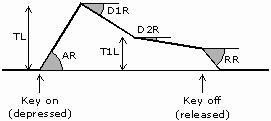
\includegraphics[width=\textwidth,height=.55\textheight,keepaspectratio]{img/envelope.png}
\caption{Chip envelope stages. TL controls the peak; T1L is the panel's
sustain level. Key on/off correspond to gate changes.}
\label{fig:envelope-generator}
\end{figure}
Choose an audible TL and fast attack before adjusting the two decays. The
second decay can continue while the key is held, so this envelope need not
settle at a constant sustain amplitude.
